\StartPlate{V04}{What a compact binder can do}{Compatible solutions in one fixed compact space can survive every precision.}
\begin{center}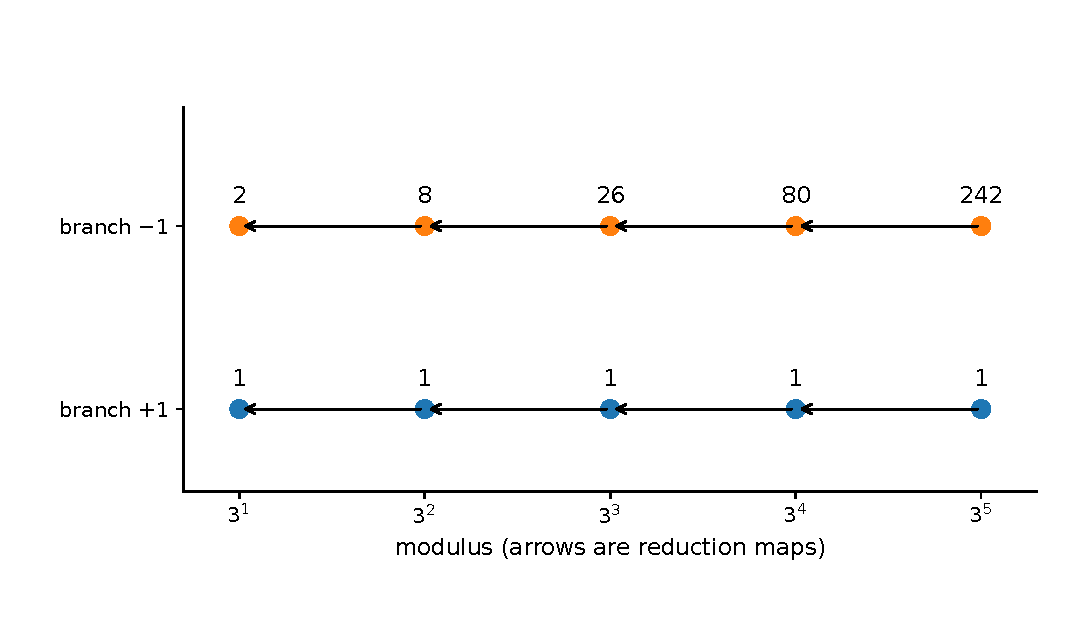
\includegraphics[width=\linewidth]{figures/V04.pdf}\end{center}
The points are all roots of $x^2-1$ modulo $3^n$, for $1\le n\le5$. The labels are canonical residue representatives. The arrows reduce a root modulo $3^n$ to a root modulo $3^{n-1}$. Both branches persist, corresponding to $1$ and $-1$ in $\Z_3$.

For the general binder, fix a closed $X\subseteq\mathcal O^m$ and continuous constraints $f_j$. The sets
\[
C_n=\{x\in X:f_j(x)\in\varpi^n\mathcal O\text{ for every }j\le n\}
\]
are closed and nested. If every $C_n$ is nonempty, compactness supplies a point satisfying every exact equation.

The example does not prove simultaneous finite solvability for the arithmetic problem. Even $x=0$ and $x=1$ have separately solvable congruences but no joint solution modulo three. Allowing the number of coefficients or pole bounds to grow also changes the compact model. Those missing hypotheses cannot be replaced by more isolated successful tests.
\vfill\PlateSource{Exact finite illustration}{Part I, Section 5; Part II, Section 19.1}{10}
